\documentclass{article}
\usepackage{float,amsmath}
\usepackage{graphicx}
\usepackage{color}
\usepackage[letterpaper,margin=1in]{geometry}
\usepackage{hyperref}

%\setlength{\textwidth}{6.5in}

\begin{document}

\author{David DeBoer}
\title{RFI Report}
\maketitle

In order to provide monitoring input of the SKA-SA Karoo Astronomy Reserve RFI environment, HERA will produce nightly RFI reports with the following structure:

\begin{itemize}
\item Filename/location of .npz file containing nightly waterfall plot flags.  Resolution is about 8 sec in time and 97 kHz in frequency
\item Nightly waterfall plot with occupancy summaries along both axes (see Fig \ref{fig:occ})
\item Occupancy plots by frequency on roughly 15 min timescales
\end{itemize}

\begin{figure}[H]
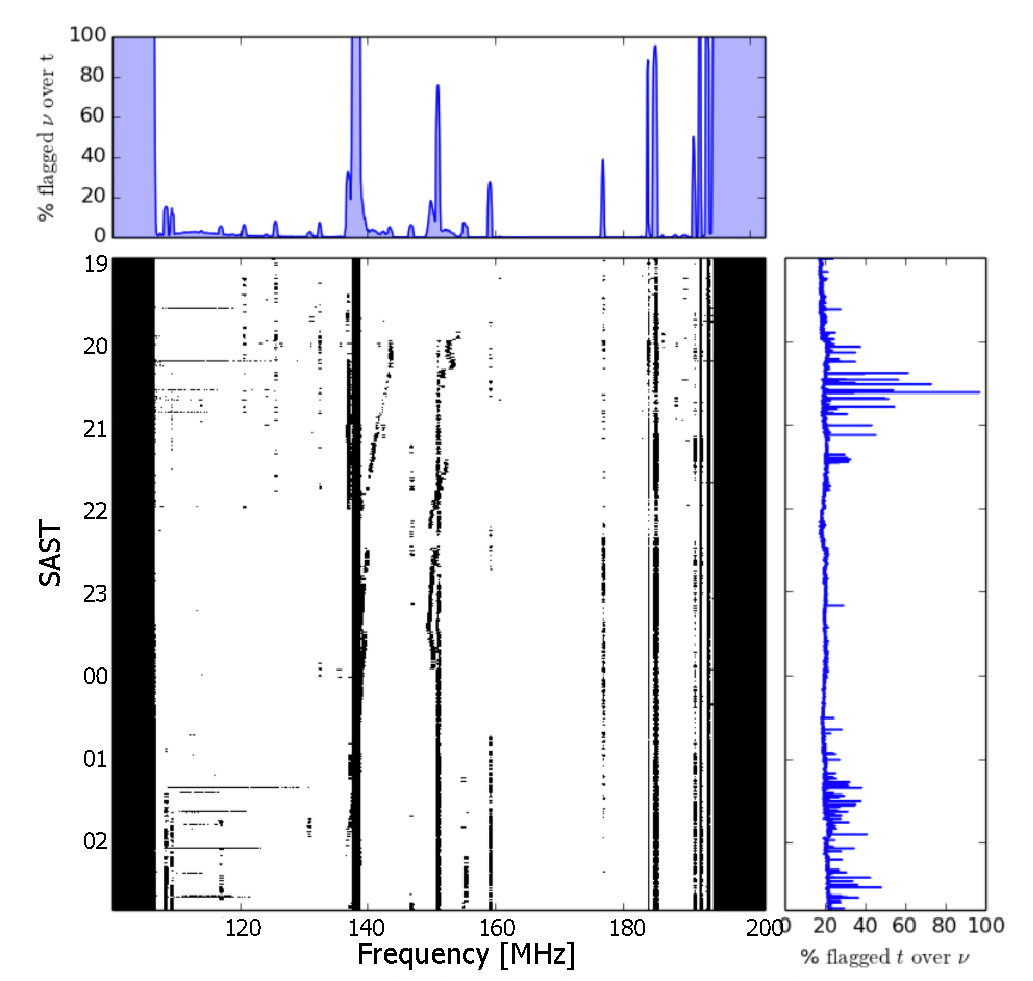
\includegraphics[width=0.5\textwidth]{report_plot.pdf}
\centering
\caption{Format of nightly overview plot.}
\label{fig:occ}
\end{figure}

For more information and discussion of the overall RFI environment see HERA Memo 7:  The HERA RFI Environment, Saul Kohn Sept 2015 (http://reionization.org/science/memos/).

\end{document}